\documentclass[10pt]{beamer}

% Modern, clean theme (built-in)
\usetheme{Madrid}
\usecolortheme{seahorse}
\usefonttheme{professionalfonts}

% Packages
\usepackage{booktabs}
\usepackage{graphicx}
\usepackage{xcolor}
\usepackage{listings}
\usepackage{tikz}
\usetikzlibrary{shapes.geometric, arrows.meta, positioning, fit, backgrounds}

% Colors
\definecolor{accent}{RGB}{0,102,204}
\definecolor{alertred}{RGB}{204,0,0}
\definecolor{successgreen}{RGB}{0,153,51}

% Code styling
\lstset{
  basicstyle=\ttfamily\footnotesize,
  breaklines=true,
  frame=single,
  backgroundcolor=\color{gray!10}
}

% Define YAML language for syntax highlighting
\lstdefinelanguage{yaml}{
  keywords={true,false,null,yes,no},
  keywordstyle=\color{blue}\bfseries,
  comment=[l]{\#},
  commentstyle=\color{gray}\itshape,
  stringstyle=\color{red},
  morestring=[b]',
  morestring=[b]",
  sensitive=false,
  moredelim=[s][\color{purple}]{:}{\ },
  literate={>}{{\textcolor{purple}{>}}}1
           {|}{{\textcolor{purple}{|}}}1
           {-}{{\textcolor{purple}{-}}}1,
}

% Title page
\title{Standardized, Reproducible Parameter Curation for QSP Models}
\subtitle{A Template-Based LLM Workflow}
\author{Joel Eliason}
\date{\today}
\institute{Johns Hopkins University}

\begin{document}

% ========================================
% TITLE SLIDE
% ========================================
\maketitle

% ========================================
% TABLE OF CONTENTS
% ========================================
\begin{frame}{Overview}
  \tableofcontents
\end{frame}

% ========================================
% SECTION 1: MOTIVATION
% ========================================
\section{The Problem}

\begin{frame}[plain,c]
  \begin{center}
    \Huge\textbf{The Problem}
  \end{center}
\end{frame}

\begin{frame}{The QSP Reproducibility Crisis}

  \begin{block}{Current State of Parameter Curation}
    QSP models require \textbf{100+ parameters} from diverse literature, but:
  \end{block}

  \vspace{0.3cm}

  \begin{itemize}
    \item \alert{Ad-hoc extraction}: No standardized methodology
    \item \alert{Poor documentation}: Values cited without context or uncertainty
    \item \alert{Propagation errors}: Parameters copied across models without verification
    \item \alert{"Telephone game" effect}: Loss of biological context and accumulating errors
    \item \alert{Difficult to verify}: Reviewers can't easily trace parameters to sources
  \end{itemize}

  \vspace{0.3cm}

  \begin{alertblock}{Result}
    Models are difficult to reproduce, validate, and reuse
  \end{alertblock}

\end{frame}

\begin{frame}{Why Standardization is Hard}

  \begin{columns}[T]
    \begin{column}{0.48\textwidth}
      \textbf{What we need:}
      \begin{itemize}
        \item Numerical values + uncertainty
        \item Biological context
        \item Experimental conditions
        \item Statistical distributions
        \item Literature provenance
        \item Cross-study synthesis
      \end{itemize}
    \end{column}

    \begin{column}{0.48\textwidth}
      \textbf{The barriers:}
      \begin{itemize}
        \item Manual curation at this level can take \alert{weeks to months}
        \item Adding documentation increases burden
        \item No widely adopted standards
        \item Trade-off: speed vs. thoroughness
      \end{itemize}
    \end{column}
  \end{columns}

  \vspace{0.5cm}

  \begin{block}{The Dilemma}
    Modelers choose \emph{speed} over standardization because comprehensive curation is too time-intensive
  \end{block}

\end{frame}

% ========================================
% SECTION 2: SOLUTION
% ========================================
\section{Our Solution}

\begin{frame}[plain,c]
  \begin{center}
    \Huge\textbf{Our Solution}
  \end{center}
\end{frame}

\begin{frame}{Template-Based LLM Workflow}

  \begin{block}{Key Insight}
    LLMs can automate extraction \textbf{while enforcing standardization} through structured templates
  \end{block}

  \vspace{0.3cm}

  \begin{columns}[T]
    \begin{column}{0.48\textwidth}
      \textbf{Innovation 1: Templates}
      \begin{itemize}
        \item YAML schemas define required metadata
        \item Enforce consistent structure
        \item Machine-parsable + human-readable
        \item Version controlled
      \end{itemize}
    \end{column}

    \begin{column}{0.48\textwidth}
      \textbf{Innovation 2: LLM Reasoning}
      \begin{itemize}
        \item Complete transparency to derivation
        \item Captures interpretation decisions
        \item Documents study selection rationale
        \item Makes expert knowledge explicit
      \end{itemize}
    \end{column}
  \end{columns}

  \vspace{0.3cm}

  \begin{exampleblock}{Goal}
    Achieve both \textcolor{successgreen}{\textbf{rigor}} AND \textcolor{successgreen}{\textbf{efficiency}} through automation
  \end{exampleblock}

\end{frame}

\begin{frame}{Six Core Metadata Dimensions}

  Our templates capture comprehensive parameter information:

  \vspace{0.3cm}

  \begin{enumerate}
    \item \textbf{Numerical values with uncertainty}
    \begin{itemize}
      \item Point estimates, ranges, confidence intervals
      \item Statistical distributions (normal, lognormal, uniform)
    \end{itemize}

    \item \textbf{Biological context}
    \begin{itemize}
      \item Species, cell types, tissue compartments
      \item Disease state and cancer type
    \end{itemize}

    \item \textbf{Experimental conditions}
    \begin{itemize}
      \item Assay type, time points, treatments
    \end{itemize}

    \item \textbf{Statistical distributions}
    \begin{itemize}
      \item Distribution parameters and R bootstrap code
    \end{itemize}

    \item \textbf{Literature provenance}
    \begin{itemize}
      \item DOI, figure/table numbers, specific passages
    \end{itemize}

    \item \textbf{Cross-study pooling methodology}
    \begin{itemize}
      \item Pooling strategy and heterogeneity assessment
    \end{itemize}
  \end{enumerate}

\end{frame}

% ========================================
% SECTION 3: SYSTEM ARCHITECTURE
% ========================================
\section{System Architecture}

\begin{frame}[plain,c]
  \begin{center}
    \Huge\textbf{System Architecture}
  \end{center}
\end{frame}

\begin{frame}{Modular Prompt Assembly System}

  \begin{center}
    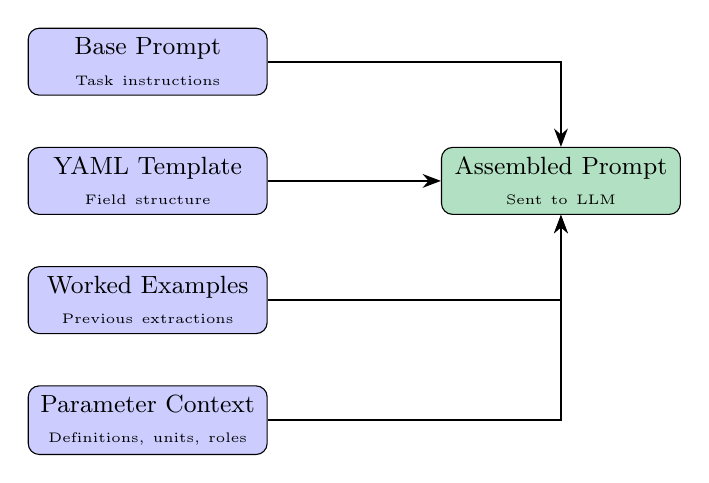
\begin{tikzpicture}[
      node distance=0.65cm,
      box/.style={rectangle, draw, fill=blue!20, text width=2.8cm, align=center, minimum height=0.85cm, rounded corners, font=\small},
      arrow/.style={-Stealth, thick}
    ]
      % Components
      \node[box] (base) {Base Prompt\\{\tiny Task instructions}};
      \node[box, below=of base] (template) {YAML Template\\{\tiny Field structure}};
      \node[box, below=of template] (examples) {Worked Examples\\{\tiny Previous extractions}};
      \node[box, below=of examples] (context) {Parameter Context\\{\tiny Definitions, units, roles}};

      % Assembly
      \node[box, fill=successgreen!30, right=2.2cm of template] (assembled) {Assembled Prompt\\{\tiny Sent to LLM}};

      % Arrows
      \draw[arrow] (base.east) -| (assembled.north);
      \draw[arrow] (template.east) -- (assembled.west);
      \draw[arrow] (examples.east) -| (assembled.south);
      \draw[arrow] (context.east) -| (assembled.south);

    \end{tikzpicture}
  \end{center}

  \vspace{0.15cm}

  \begin{itemize}
    \item \textbf{Modular} components, \textbf{configurable} via YAML
    \item \textbf{Reusable} across workflows, \textbf{maintainable} centrally
  \end{itemize}

\end{frame}

\begin{frame}{Three Workflow Types}

  \begin{block}{1. Parameter Extraction}
    \textbf{Purpose}: Detailed metadata with full provenance\\
    \textbf{Output}: All six metadata dimensions\\
    \textbf{Use case}: Publication-ready parameter curation
  \end{block}

  \vspace{0.2cm}

  \begin{block}{2. Quick Estimates}
    \textbf{Purpose}: Rapid parameter initialization\\
    \textbf{Output}: Ballpark values and ranges\\
    \textbf{Use case}: Early-stage model testing
  \end{block}

  \vspace{0.2cm}

  \begin{block}{3. Test Statistics}
    \textbf{Purpose}: Validation targets from experimental data\\
    \textbf{Output}: Statistical distributions with R bootstrap code\\
    \textbf{Use case}: Model validation and calibration
  \end{block}

\end{frame}

\begin{frame}[fragile]{Data Flow: Literature → YAML}

  \begin{center}
    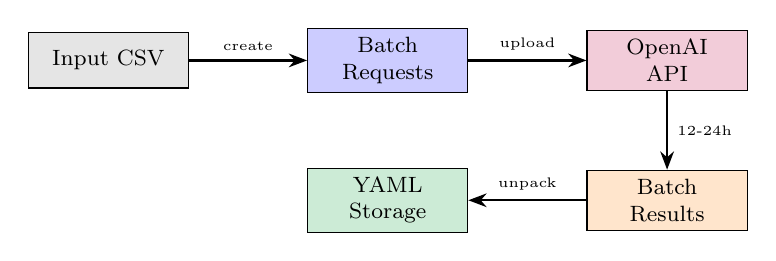
\begin{tikzpicture}[
      node distance=1.5cm,
      box/.style={rectangle, draw, text width=1.8cm, align=center, minimum height=0.7cm, font=\footnotesize},
      arrow/.style={-Stealth, thick}
    ]
      % Top row: Input → Batch → API
      \node[box, fill=gray!20] (csv) {Input CSV};
      \node[box, fill=blue!20, right=of csv] (batch) {Batch\\Requests};
      \node[box, fill=purple!20, right=of batch] (api) {OpenAI\\API};

      % Bottom row: Results → YAML (flowing back)
      \node[box, fill=orange!20, below=1cm of api] (results) {Batch\\Results};
      \node[box, fill=successgreen!20, left=of results] (yaml) {YAML\\Storage};

      % Arrows
      \draw[arrow] (csv) -- (batch) node[midway, above, font=\tiny] {create};
      \draw[arrow] (batch) -- (api) node[midway, above, font=\tiny] {upload};
      \draw[arrow] (api) -- (results) node[midway, right, font=\tiny] {12-24h};
      \draw[arrow] (results) -- (yaml) node[midway, above, font=\tiny] {unpack};

    \end{tikzpicture}
  \end{center}

  \vspace{0.3cm}

  \begin{itemize}
    \item \textbf{Batch API}: 50\% cost savings, async processing (12-24h)
    \item \textbf{Output}: Version-controlled YAML files in flat structure
    \item \textbf{Naming}: \texttt{\{param\}\_\{author\}\_\{cancer\}\_\{hash\}.yaml}
    \begin{itemize}
      \item Hash computed from study context enables multiple extractions per parameter
    \end{itemize}
  \end{itemize}

\end{frame}

\begin{frame}[fragile]{Example: YAML Output}

  \begin{lstlisting}[language=yaml, basicstyle=\ttfamily\tiny]
parameter_name: "ki67_tumor_proliferation_rate"
canonical_scale: "log"
parameter_estimate:
  value: 0.0048
  unit: "1/h"
  type: "lognormal"
  confidence_interval: [0.0032, 0.0067]
biological_context:
  species: "human"
  cell_type: "PDAC tumor cells"
  disease_state: "pancreatic ductal adenocarcinoma"
experimental_design:
  assay_type: "Ki-67 immunohistochemistry"
  measurement_type: "proliferation index"
  sample_size: 156
statistical_distribution:
  distribution_family: "lognormal"
  parameters: {meanlog: -5.34, sdlog: 0.18}
  r_bootstrap_code: |
    rlnorm(n, meanlog=-5.34, sdlog=0.18)
sources:
  - citation: "Smith et al. (2020)"
    doi: "10.1234/example"
    figure_or_table: "Figure 3B"
    specific_passage: "Median Ki-67 index was 48%..."
  \end{lstlisting}

  \textbf{Complete, standardized, machine-parsable metadata!}

\end{frame}

% ========================================
% SECTION 4: RESULTS & VALIDATION PLAN
% ========================================
\section{Current Progress \& Validation Plan}

\begin{frame}[plain,c]
  \begin{center}
    \Huge\textbf{Current Progress}\\
    \Huge\textbf{\& Validation Plan}
  \end{center}
\end{frame}

\begin{frame}{PDAC Application: Prototype Status}

  \begin{block}{Model Context}
    Pancreatic ductal adenocarcinoma (PDAC) tumor microenvironment model\\
    Therapeutic targets: checkpoint inhibitors, chemotherapy combinations
  \end{block}

  \vspace{0.3cm}

  \begin{alertblock}{Current Status: Prototype Workflow}
    \textbf{$\sim$20 parameters} trialed through complete workflow\\
    All core components functional, \textbf{but validation still needed}
  \end{alertblock}

  \vspace{0.3cm}

  \textbf{What's Working:}
  \begin{itemize}
    \item Template-guided extraction producing structured YAML
    \item Modular prompt assembly system
    \item Two-stage LLM review (extraction + automated validation)
    \item Batch processing with 12-24h turnaround
    \item Flat-file storage with version control
  \end{itemize}

\end{frame}

\begin{frame}{Key Resource: Legacy Parameter Database}

  \begin{block}{Existing Asset}
    Extensive database of manually-curated parameters from prior QSP models\\
    \textbf{Format}: Legacy YAML files with parameter values and metadata
  \end{block}

  \vspace{0.3cm}

  \textbf{Primary use for this study:}
  \begin{itemize}
    \item \textbf{Validation ground truth}: Test LLM extraction accuracy at scale (50-100+ parameters)
    \item No new expert curation required
  \end{itemize}

  \vspace{0.3cm}

  \textbf{Secondary benefits:}
  \begin{itemize}
    \item Contextualize PDAC parameters within broader QSP landscape
    \item Identify parameter patterns and coverage gaps across models
  \end{itemize}

  \vspace{0.3cm}

  \begin{alertblock}{Key advantage}
    Large-scale validation without the time/cost of new expert curation
  \end{alertblock}

\end{frame}

\begin{frame}{Primary Validation: Database Comparison}

  \textbf{Approach:} Compare LLM-extracted PDAC parameters to legacy manual curations

  \vspace{0.3cm}

  \textbf{Validation metrics:}
  \begin{itemize}
    \item Value agreement (correlation, fold-difference)
    \item Uncertainty quantification consistency
    \item Metadata completeness comparison
    \item Extraction accuracy rate
  \end{itemize}

  \vspace{0.3cm}

  \textbf{Scale:} 50-100+ overlapping parameters

  \vspace{0.3cm}

  \textbf{Bonus insights from database comparison:}
  \begin{itemize}
    \item PDAC parameter landscape contextualized with other models
    \item Cross-model parameter variability characterization
    \item Coverage gap identification
  \end{itemize}

  \vspace{0.2cm}

  \begin{alertblock}{Goal}
    Demonstrate LLM workflow produces accurate, reliable parameter metadata
  \end{alertblock}

\end{frame}

\begin{frame}{Complementary Validation Options}

  \textbf{Additional validation to strengthen the study (optional):}

  \vspace{0.3cm}

  \begin{block}{Option A: Expert Comparison for Gap Parameters}
    \textbf{Use case:} Parameters NOT in legacy database\\
    \textbf{Approach:} Expert manually curates 10-20 parameters using identical sources\\
    \textbf{Benefit:} Fills database coverage gaps + time savings measurement\\
    \textbf{Effort:} High (requires expert time)
  \end{block}

  \vspace{0.3cm}

  \begin{block}{Option B: Downstream Model Performance}
    \textbf{Use case:} If PDAC model ready for testing\\
    \textbf{Approach:} Use LLM parameters in model, compare predictions to data\\
    \textbf{Benefit:} Real-world utility demonstration\\
    \textbf{Effort:} Medium (depends on model readiness)
  \end{block}

\end{frame}

\begin{frame}{Implemented: Two-Stage LLM Review}

  \begin{columns}[T]
    \begin{column}{0.48\textwidth}
      \textbf{Stage 1: Extraction}
      \begin{itemize}
        \item Reads literature
        \item Fills YAML template
        \item Provides reasoning trace
      \end{itemize}
    \end{column}

    \begin{column}{0.48\textwidth}
      \textbf{Stage 2: Review}
      \begin{itemize}
        \item 54-item checklist
        \item Citation verification
        \item Hallucination detection
        \item Returns corrected JSON
      \end{itemize}
    \end{column}
  \end{columns}

  \vspace{0.2cm}

  \begin{block}{Checklist covers:}
    Parameter accuracy, statistical rigor, experimental design, source validation, formatting standards
  \end{block}

  \vspace{0.2cm}

  \begin{alertblock}{Goal}
    Reduce expert burden while catching errors before manual validation
  \end{alertblock}

\end{frame}

% ========================================
% SECTION 5: PAPER COLLABORATION
% ========================================
\section{Paper Collaboration}

\begin{frame}[plain,c]
  \begin{center}
    \Huge\textbf{Paper Collaboration}
  \end{center}
\end{frame}

\begin{frame}{Current Status}

  \begin{columns}[T]
    \begin{column}{0.48\textwidth}
      \textcolor{successgreen}{\textbf{Completed}}
      \begin{itemize}
        \item[\checkmark] Core workflows implemented
        \item[\checkmark] Prototype tested (~20 parameters)
        \item[\checkmark] YAML templates finalized (v2)
        \item[\checkmark] LLM review system (54-item)
        \item[\checkmark] Flat-file storage system
        \item[\checkmark] Paper outline drafted
        \item[\checkmark] Onboarding materials prepared
      \end{itemize}
    \end{column}

    \begin{column}{0.48\textwidth}
      \textbf{Remaining}
      \begin{itemize}
        \item[$\square$] Finalize validation approach
        \item[$\square$] Database comparison validation analysis
        \item[$\square$] Complementary validation (if needed)
        \item[$\square$] Generate figures/tables
        \item[$\square$] Write manuscript
        \item[$\square$] Supplementary materials
        \item[$\square$] Code release prep
      \end{itemize}
    \end{column}
  \end{columns}

\end{frame}

\begin{frame}{Repository Organization}

  \begin{block}{This repository: \texttt{qsp-llm-workflows}}
    General-purpose LLM workflow tools for parameter extraction\\
    \textbf{Scope}: Reusable across any QSP model or disease area
  \end{block}

  \vspace{0.3cm}

  \begin{block}{Paper repository: \texttt{qsp-llm-workflows-paper} (to be created)}
    Paper-specific code, validation analyses, and figures\\
    \textbf{Scope}: Validation study, results analysis, manuscript figures
  \end{block}

  \vspace{0.3cm}

  \textbf{Benefits:}
  \begin{itemize}
    \item Clean separation between general tools and paper-specific work
    \item This repo remains focused and reusable
    \item Paper repo contains reproducible analyses for publication
  \end{itemize}

\end{frame}

\begin{frame}{What We Need: Division of Labor}

  \textbf{Areas for collaboration (to discuss):}

  \vspace{0.3cm}

  \begin{enumerate}
    \item \textbf{Database Comparison Validation}
    \begin{itemize}
      \item Align LLM extractions with legacy YAML parameters
      \item Compute validation metrics (correlation, agreement, metadata quality)
      \item Statistical analysis scripting
      \item Contextualization: PDAC parameters vs. other models (secondary analysis)
    \end{itemize}

    \item \textbf{Complementary Validation} (if needed)
    \begin{itemize}
      \item Expert curation for gap parameters
      \item Time tracking and efficiency metrics
    \end{itemize}

    \item \textbf{Writing \& Figures}
    \begin{itemize}
      \item Methods (workflow, templates, validation approach)
      \item Results (validation metrics, contextualized findings)
      \item Discussion (workflow accuracy, reproducibility, generalizability)
      \item Figures: validation plots, metadata quality comparisons
    \end{itemize}

    \item \textbf{Supplementary Materials}
    \begin{itemize}
      \item Complete template specifications
      \item LLM reviewer documentation
      \item Code repository preparation
    \end{itemize}
  \end{enumerate}

\end{frame}

\begin{frame}{Proposed Timeline}

  \begin{table}
    \centering
    \small
    \begin{tabular}{lp{6cm}}
      \toprule
      \textbf{Timeframe} & \textbf{Milestones} \\
      \midrule
      \textbf{Week 1-3} & Database comparison validation\\
                        & Align extractions, compute metrics, contextualize with other models \\
      \midrule
      \textbf{Week 4-5} & Complementary validation (if needed)\\
                        & Gap parameter expert curation, time tracking \\
      \midrule
      \textbf{Week 6-7} & Figure generation and results analysis\\
                        & Validation plots, metadata quality comparisons \\
      \midrule
      \textbf{Week 8-9} & Manuscript drafting\\
                        & All sections, supplementary materials \\
      \midrule
      \textbf{Week 10} & Revisions and submission prep\\
                        & Internal review, final polishing \\
      \bottomrule
    \end{tabular}
  \end{table}

  \vspace{0.3cm}

  \textbf{Target journal}: \emph{CPT: Pharmacometrics \& Systems Pharmacology}

  \vspace{0.2cm}

  \textcolor{gray}{\footnotesize Timeline is preliminary and subject to discussion}

\end{frame}

% ========================================
% SECTION 6: GETTING STARTED
% ========================================
\section{Next Steps}

\begin{frame}[plain,c]
  \begin{center}
    \Huge\textbf{Next Steps}
  \end{center}
\end{frame}

\begin{frame}{Getting Started Today}

  \textbf{Environment setup (5 minutes):}
  \begin{enumerate}
    \item Activate virtual environment: \texttt{source venv/bin/activate}
    \item Add API key to \texttt{.env}: \texttt{OPENAI\_API\_KEY=sk-...}
    \item Clone sister repo: \texttt{qsp-metadata-storage}
  \end{enumerate}

  \vspace{0.3cm}

  \textbf{Explore the codebase:}
  \begin{itemize}
    \item Read: \texttt{docs/COLLABORATOR\_ONBOARDING.md} (comprehensive guide)
    \item Review: \texttt{scratch/paper\_outline\_standardization.md}
    \item Browse: Existing extractions in \texttt{qsp-metadata-storage/}
    \item Try: Run a quick estimate workflow on a test parameter
  \end{itemize}

  \vspace{0.3cm}

  \textbf{Key documentation:}
  \begin{itemize}
    \item \texttt{CLAUDE.md}: Complete codebase reference
    \item \texttt{templates/*.yaml}: See our schemas
    \item \texttt{prompts/*.md}: See how we prompt LLMs
  \end{itemize}

\end{frame}

\begin{frame}{Immediate Action Items}

  \textbf{This week:}
  \begin{enumerate}
    \item \checkmark Attend this presentation / discussion
    \item $\square$ Review paper outline and decide on roles
    \item $\square$ Set up development environment
    \item $\square$ Run a test extraction workflow
    \item $\square$ Identify questions and areas needing clarification
  \end{enumerate}

  \vspace{0.5cm}

  \textbf{By next meeting:}
  \begin{enumerate}
    \item $\square$ Finalize validation study design
    \item $\square$ Assign paper sections and figures
    \item $\square$ Create task tracking system (GitHub issues/project)
    \item $\square$ Schedule regular collaboration meetings
  \end{enumerate}

  \vspace{0.5cm}

  \begin{center}
    \Large\textbf{Let's discuss roles and next steps!}
  \end{center}

\end{frame}

% ========================================
% FINAL SLIDE
% ========================================
\begin{frame}[plain,c]

  \begin{center}
    \Huge Thank You!

    \vspace{1cm}

    \Large Questions \& Discussion

    \vspace{1cm}

    \normalsize
    \textit{Onboarding guide \& paper outline}\\
    \textit{(shared via email)}
  \end{center}

\end{frame}

\end{document}
